\chapter{路径与回路}

本章重点讨论图中的两类路径：
\begin{itemize}
\item \key{欧拉路径}是恰好经过每条边一次的路径。
\item \key{哈密顿路径}是恰好访问每个结点一次的路径。
\end{itemize}

欧拉路径和哈密顿路径乍看之下十分相似，但与它们有关的计算问题却截然不同。判断一个图是否包含欧拉路径有一条简单的规则，而且如果欧拉路径存在，也有高效算法能够找到它。相反，判断哈密顿路径是否存在是一个 NP 困难问题，目前没有已知的高效算法。

\section{欧拉路径}

\index{Eulerian path}

\key{欧拉路径}\footnote{L. Euler 于 1736 年研究了这类路径，并解决了著名的柯尼斯堡七桥问题。这也标志着图论的诞生。}是恰好经过图中每条边一次的路径。例如，图
\begin{center}
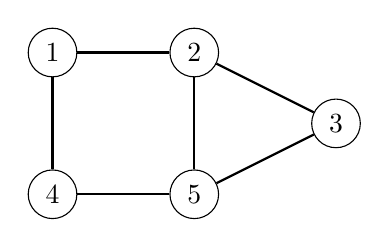
\begin{tikzpicture}[scale=0.9]
\node[draw, circle] (1) at (1,5) {$1$};
\node[draw, circle] (2) at (3,5) {$2$};
\node[draw, circle] (3) at (5,4) {$3$};
\node[draw, circle] (4) at (1,3) {$4$};
\node[draw, circle] (5) at (3,3) {$5$};

\path[draw,thick,-] (1) -- (2);
\path[draw,thick,-] (2) -- (3);
\path[draw,thick,-] (1) -- (4);
\path[draw,thick,-] (3) -- (5);
\path[draw,thick,-] (2) -- (5);
\path[draw,thick,-] (4) -- (5);
\end{tikzpicture}
\end{center}

包含一条从结点 2 到结点 5 的欧拉路径：
\begin{center}
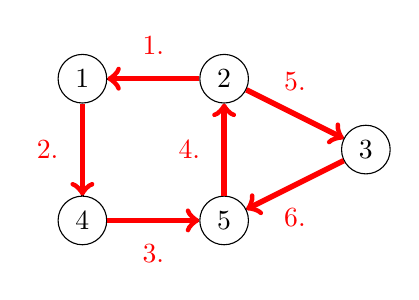
\begin{tikzpicture}[scale=0.9]
\node[draw, circle] (1) at (1,5) {$1$};
\node[draw, circle] (2) at (3,5) {$2$};
\node[draw, circle] (3) at (5,4) {$3$};
\node[draw, circle] (4) at (1,3) {$4$};
\node[draw, circle] (5) at (3,3) {$5$};

\path[draw,thick,-] (1) -- (2);
\path[draw,thick,-] (2) -- (3);
\path[draw,thick,-] (1) -- (4);
\path[draw,thick,-] (3) -- (5);
\path[draw,thick,-] (2) -- (5);
\path[draw,thick,-] (4) -- (5);

\path[draw=red,thick,->,line width=2pt] (2) -- node[font=\small,label={[red]north:1.}] {} (1);
\path[draw=red,thick,->,line width=2pt] (1) -- node[font=\small,label={[red]left:2.}] {} (4);
\path[draw=red,thick,->,line width=2pt] (4) -- node[font=\small,label={[red]south:3.}] {} (5);
\path[draw=red,thick,->,line width=2pt] (5) -- node[font=\small,label={[red]left:4.}] {} (2);
\path[draw=red,thick,->,line width=2pt] (2) -- node[font=\small,label={[red]north:5.}] {} (3);
\path[draw=red,thick,->,line width=2pt] (3) -- node[font=\small,label={[red]south:6.}] {} (5);
\end{tikzpicture}
\end{center}
\index{Eulerian circuit}
起点和终点为同一结点的欧拉路径称为\key{欧拉回路}。例如，图
\begin{center}
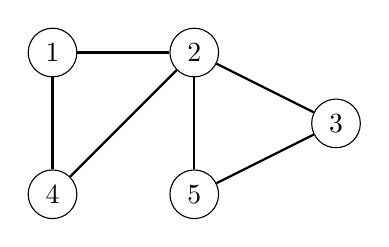
\begin{tikzpicture}[scale=0.9]
\node[draw, circle] (1) at (1,5) {$1$};
\node[draw, circle] (2) at (3,5) {$2$};
\node[draw, circle] (3) at (5,4) {$3$};
\node[draw, circle] (4) at (1,3) {$4$};
\node[draw, circle] (5) at (3,3) {$5$};

\path[draw,thick,-] (1) -- (2);
\path[draw,thick,-] (2) -- (3);
\path[draw,thick,-] (1) -- (4);
\path[draw,thick,-] (3) -- (5);
\path[draw,thick,-] (2) -- (5);
\path[draw,thick,-] (2) -- (4);
\end{tikzpicture}
\end{center}
包含一条以结点 1 为起点和终点的欧拉回路：
\begin{center}
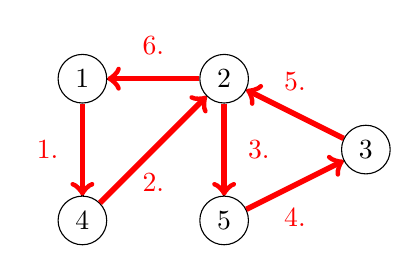
\begin{tikzpicture}[scale=0.9]
\node[draw, circle] (1) at (1,5) {$1$};
\node[draw, circle] (2) at (3,5) {$2$};
\node[draw, circle] (3) at (5,4) {$3$};
\node[draw, circle] (4) at (1,3) {$4$};
\node[draw, circle] (5) at (3,3) {$5$};

\path[draw,thick,-] (1) -- (2);
\path[draw,thick,-] (2) -- (3);
\path[draw,thick,-] (1) -- (4);
\path[draw,thick,-] (3) -- (5);
\path[draw,thick,-] (2) -- (5);
\path[draw,thick,-] (2) -- (4);

\path[draw=red,thick,->,line width=2pt] (1) -- node[font=\small,label={[red]left:1.}] {} (4);
\path[draw=red,thick,->,line width=2pt] (4) -- node[font=\small,label={[red]south:2.}] {} (2);
\path[draw=red,thick,->,line width=2pt] (2) -- node[font=\small,label={[red]right:3.}] {} (5);
\path[draw=red,thick,->,line width=2pt] (5) -- node[font=\small,label={[red]south:4.}] {} (3);
\path[draw=red,thick,->,line width=2pt] (3) -- node[font=\small,label={[red]north:5.}] {} (2);
\path[draw=red,thick,->,line width=2pt] (2) -- node[font=\small,label={[red]north:6.}] {} (1);
\end{tikzpicture}
\end{center}

\subsubsection{存在条件}

欧拉路径和欧拉回路是否存在，取决于各结点的度。首先，无向图恰好在所有边都属于同一个连通分量，并且满足以下条件之一时存在欧拉路径：
\begin{itemize}
\item 每个结点的度均为偶数；\emph{或}
\item 恰有两个结点的度为奇数，其余结点的度均为偶数。
\end{itemize}

第一种情况下，每条欧拉路径也都是欧拉回路。第二种情况下，两个奇度结点分别是某条非欧拉回路的欧拉路径的起点和终点。

\begin{samepage}
例如，在图
\begin{center}
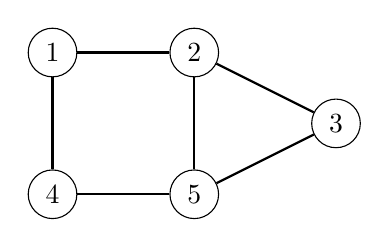
\begin{tikzpicture}[scale=0.9]
\node[draw, circle] (1) at (1,5) {$1$};
\node[draw, circle] (2) at (3,5) {$2$};
\node[draw, circle] (3) at (5,4) {$3$};
\node[draw, circle] (4) at (1,3) {$4$};
\node[draw, circle] (5) at (3,3) {$5$};

\path[draw,thick,-] (1) -- (2);
\path[draw,thick,-] (2) -- (3);
\path[draw,thick,-] (1) -- (4);
\path[draw,thick,-] (3) -- (5);
\path[draw,thick,-] (2) -- (5);
\path[draw,thick,-] (4) -- (5);
\end{tikzpicture}
\end{center}
\end{samepage}
中，结点 1、3、4 的度为 2，结点 2、5 的度为 3。恰有两个结点的度为奇数，因此结点 2 与结点 5 之间存在欧拉路径，但该图不包含欧拉回路。

对于有向图，我们考察结点的入度与出度。有向图恰好在所有边都属于同一个连通分量，并且满足以下条件之一时包含欧拉路径：
\begin{itemize}
\item 每个结点的入度都等于出度；\emph{或}
\item 有一个结点的入度比出度大 1，另一个结点的出度比入度大 1，其余结点的入度都等于出度。
\end{itemize}

第一种情况下，每条欧拉路径也都是欧拉回路；第二种情况下，图中存在一条欧拉路径，它从出度较大的结点出发，在入度较大的结点结束。

例如，在图
\begin{center}
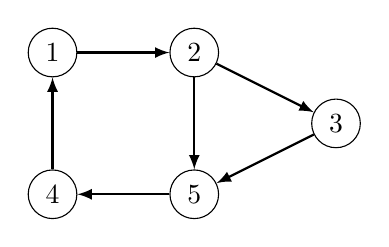
\begin{tikzpicture}[scale=0.9]
\node[draw, circle] (1) at (1,5) {$1$};
\node[draw, circle] (2) at (3,5) {$2$};
\node[draw, circle] (3) at (5,4) {$3$};
\node[draw, circle] (4) at (1,3) {$4$};
\node[draw, circle] (5) at (3,3) {$5$};

\path[draw,thick,->,>=latex] (1) -- (2);
\path[draw,thick,->,>=latex] (2) -- (3);
\path[draw,thick,->,>=latex] (4) -- (1);
\path[draw,thick,->,>=latex] (3) -- (5);
\path[draw,thick,->,>=latex] (2) -- (5);
\path[draw,thick,->,>=latex] (5) -- (4);
\end{tikzpicture}
\end{center}
中，结点 1、3、4 的入度和出度均为 1，结点 2 的入度为 1、出度为 2，结点 5 的入度为 2、出度为 1。因此，该图包含一条从结点 2 到结点 5 的欧拉路径：
\begin{center}
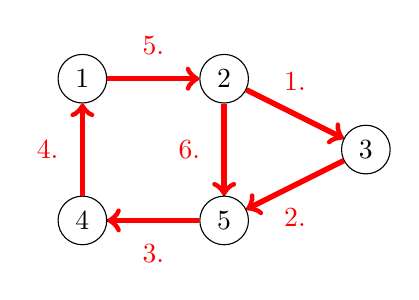
\begin{tikzpicture}[scale=0.9]
\node[draw, circle] (1) at (1,5) {$1$};
\node[draw, circle] (2) at (3,5) {$2$};
\node[draw, circle] (3) at (5,4) {$3$};
\node[draw, circle] (4) at (1,3) {$4$};
\node[draw, circle] (5) at (3,3) {$5$};

\path[draw,thick,-] (1) -- (2);
\path[draw,thick,-] (2) -- (3);
\path[draw,thick,-] (1) -- (4);
\path[draw,thick,-] (3) -- (5);
\path[draw,thick,-] (2) -- (5);
\path[draw,thick,-] (4) -- (5);

\path[draw=red,thick,->,line width=2pt] (2) -- node[font=\small,label={[red]north:1.}] {} (3);
\path[draw=red,thick,->,line width=2pt] (3) -- node[font=\small,label={[red]south:2.}] {} (5);
\path[draw=red,thick,->,line width=2pt] (5) -- node[font=\small,label={[red]south:3.}] {} (4);
\path[draw=red,thick,->,line width=2pt] (4) -- node[font=\small,label={[red]left:4.}] {} (1);
\path[draw=red,thick,->,line width=2pt] (1) -- node[font=\small,label={[red]north:5.}] {} (2);
\path[draw=red,thick,->,line width=2pt] (2) -- node[font=\small,label={[red]left:6.}] {} (5);
\end{tikzpicture}
\end{center}

\subsubsection{Hierholzer 算法}

\index{Hierholzer's algorithm}

\key{Hierholzer 算法}\footnote{该算法于 1873 年在 Hierholzer 去世后发表 \cite{hie73}。}是一种构造欧拉回路的高效方法。算法分若干轮执行，每一轮都向回路中加入一些新边。当然，我们假设图中包含欧拉回路；否则 Hierholzer 算法不可能找到它。

首先，算法构造一个包含图中部分边（不一定是全部边）的回路。随后，算法逐步向该回路中插入子回路，以扩展原回路。这个过程持续到所有边都被加入回路为止。

扩展回路时，算法总是寻找一个属于当前回路、但仍有某条出边尚未包含在回路中的结点 $x$。然后从结点 $x$ 出发，仅沿尚未加入回路的边构造一条新路径。这条路径迟早会返回结点 $x$，从而形成一个子回路。

如果图中只有欧拉路径，我们仍可利用 Hierholzer 算法寻找它：先向图中加入一条额外的边，构造出欧拉回路后再删去这条边。例如，在无向图中，可在两个奇度结点之间加入这条额外边。

下面考察 Hierholzer 算法如何为一个无向图构造欧拉回路。
\subsubsection{示例}

\begin{samepage}
考虑下图：
\begin{center}
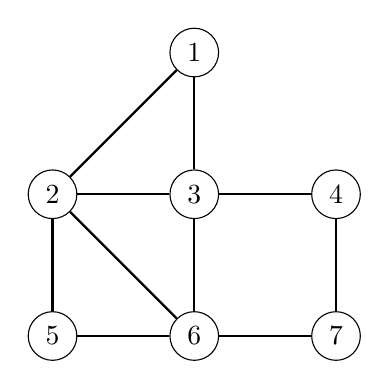
\begin{tikzpicture}[scale=0.9]
\node[draw, circle] (1) at (3,5) {$1$};
\node[draw, circle] (2) at (1,3) {$2$};
\node[draw, circle] (3) at (3,3) {$3$};
\node[draw, circle] (4) at (5,3) {$4$};
\node[draw, circle] (5) at (1,1) {$5$};
\node[draw, circle] (6) at (3,1) {$6$};
\node[draw, circle] (7) at (5,1) {$7$};

\path[draw,thick,-] (1) -- (2);
\path[draw,thick,-] (1) -- (3);
\path[draw,thick,-] (2) -- (3);
\path[draw,thick,-] (2) -- (5);
\path[draw,thick,-] (2) -- (6);
\path[draw,thick,-] (3) -- (4);
\path[draw,thick,-] (3) -- (6);
\path[draw,thick,-] (4) -- (7);
\path[draw,thick,-] (5) -- (6);
\path[draw,thick,-] (6) -- (7);
\end{tikzpicture}
\end{center}
\end{samepage}

\begin{samepage}
假设算法首先构造一条从结点 1 开始的回路。一种可能的回路是
$1 \rightarrow 2 \rightarrow 3 \rightarrow 1$：
\begin{center}
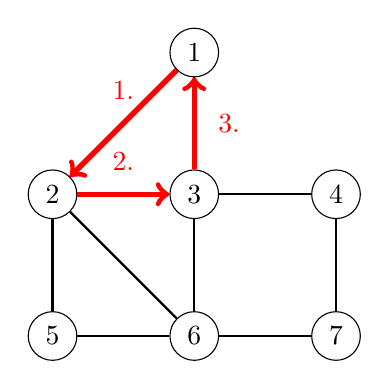
\begin{tikzpicture}[scale=0.9]
\node[draw, circle] (1) at (3,5) {$1$};
\node[draw, circle] (2) at (1,3) {$2$};
\node[draw, circle] (3) at (3,3) {$3$};
\node[draw, circle] (4) at (5,3) {$4$};
\node[draw, circle] (5) at (1,1) {$5$};
\node[draw, circle] (6) at (3,1) {$6$};
\node[draw, circle] (7) at (5,1) {$7$};

\path[draw,thick,-] (1) -- (2);
\path[draw,thick,-] (1) -- (3);
\path[draw,thick,-] (2) -- (3);
\path[draw,thick,-] (2) -- (5);
\path[draw,thick,-] (2) -- (6);
\path[draw,thick,-] (3) -- (4);
\path[draw,thick,-] (3) -- (6);
\path[draw,thick,-] (4) -- (7);
\path[draw,thick,-] (5) -- (6);
\path[draw,thick,-] (6) -- (7);

\path[draw=red,thick,->,line width=2pt] (1) -- node[font=\small,label={[red]north:1.}] {} (2);
\path[draw=red,thick,->,line width=2pt] (2) -- node[font=\small,label={[red]north:2.}] {} (3);
\path[draw=red,thick,->,line width=2pt] (3) -- node[font=\small,label={[red]east:3.}] {} (1);
\end{tikzpicture}
\end{center}
\end{samepage}
随后，算法把子回路
$2 \rightarrow 5 \rightarrow 6 \rightarrow 2$
加入当前回路：
\begin{center}
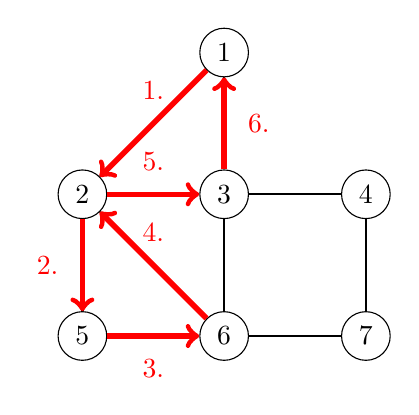
\begin{tikzpicture}[scale=0.9]
\node[draw, circle] (1) at (3,5) {$1$};
\node[draw, circle] (2) at (1,3) {$2$};
\node[draw, circle] (3) at (3,3) {$3$};
\node[draw, circle] (4) at (5,3) {$4$};
\node[draw, circle] (5) at (1,1) {$5$};
\node[draw, circle] (6) at (3,1) {$6$};
\node[draw, circle] (7) at (5,1) {$7$};

\path[draw,thick,-] (1) -- (2);
\path[draw,thick,-] (1) -- (3);
\path[draw,thick,-] (2) -- (3);
\path[draw,thick,-] (2) -- (5);
\path[draw,thick,-] (2) -- (6);
\path[draw,thick,-] (3) -- (4);
\path[draw,thick,-] (3) -- (6);
\path[draw,thick,-] (4) -- (7);
\path[draw,thick,-] (5) -- (6);
\path[draw,thick,-] (6) -- (7);

\path[draw=red,thick,->,line width=2pt] (1) -- node[font=\small,label={[red]north:1.}] {} (2);
\path[draw=red,thick,->,line width=2pt] (2) -- node[font=\small,label={[red]west:2.}] {} (5);
\path[draw=red,thick,->,line width=2pt] (5) -- node[font=\small,label={[red]south:3.}] {} (6);
\path[draw=red,thick,->,line width=2pt] (6) -- node[font=\small,label={[red]north:4.}] {} (2);
\path[draw=red,thick,->,line width=2pt] (2) -- node[font=\small,label={[red]north:5.}] {} (3);
\path[draw=red,thick,->,line width=2pt] (3) -- node[font=\small,label={[red]east:6.}] {} (1);
\end{tikzpicture}
\end{center}
最后，算法把子回路
$6 \rightarrow 3 \rightarrow 4 \rightarrow 7 \rightarrow 6$
加入当前回路：
\begin{center}
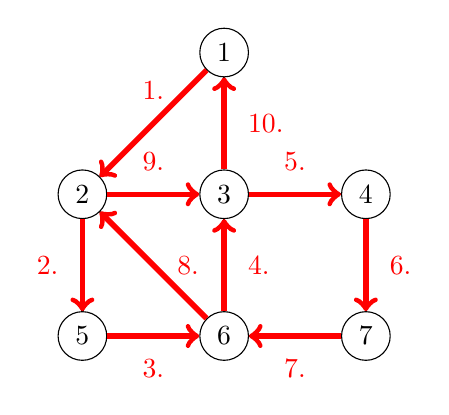
\begin{tikzpicture}[scale=0.9]
\node[draw, circle] (1) at (3,5) {$1$};
\node[draw, circle] (2) at (1,3) {$2$};
\node[draw, circle] (3) at (3,3) {$3$};
\node[draw, circle] (4) at (5,3) {$4$};
\node[draw, circle] (5) at (1,1) {$5$};
\node[draw, circle] (6) at (3,1) {$6$};
\node[draw, circle] (7) at (5,1) {$7$};

\path[draw,thick,-] (1) -- (2);
\path[draw,thick,-] (1) -- (3);
\path[draw,thick,-] (2) -- (3);
\path[draw,thick,-] (2) -- (5);
\path[draw,thick,-] (2) -- (6);
\path[draw,thick,-] (3) -- (4);
\path[draw,thick,-] (3) -- (6);
\path[draw,thick,-] (4) -- (7);
\path[draw,thick,-] (5) -- (6);
\path[draw,thick,-] (6) -- (7);

\path[draw=red,thick,->,line width=2pt] (1) -- node[font=\small,label={[red]north:1.}] {} (2);
\path[draw=red,thick,->,line width=2pt] (2) -- node[font=\small,label={[red]west:2.}] {} (5);
\path[draw=red,thick,->,line width=2pt] (5) -- node[font=\small,label={[red]south:3.}] {} (6);
\path[draw=red,thick,->,line width=2pt] (6) -- node[font=\small,label={[red]east:4.}] {} (3);
\path[draw=red,thick,->,line width=2pt] (3) -- node[font=\small,label={[red]north:5.}] {} (4);
\path[draw=red,thick,->,line width=2pt] (4) -- node[font=\small,label={[red]east:6.}] {} (7);
\path[draw=red,thick,->,line width=2pt] (7) -- node[font=\small,label={[red]south:7.}] {} (6);
\path[draw=red,thick,->,line width=2pt] (6) -- node[font=\small,label={[red]right:8.}] {} (2);
\path[draw=red,thick,->,line width=2pt] (2) -- node[font=\small,label={[red]north:9.}] {} (3);
\path[draw=red,thick,->,line width=2pt] (3) -- node[font=\small,label={[red]east:10.}] {} (1);
\end{tikzpicture}
\end{center}
此时所有边都已包含在回路中，因此我们成功构造出了一条欧拉回路。

\section{哈密顿路径}

\index{Hamiltonian path}

\key{哈密顿路径}
%\footnote{W. R. Hamilton (1805--1865) was an Irish mathematician.}
是恰好访问图中每个结点一次的路径。例如，图
\begin{center}
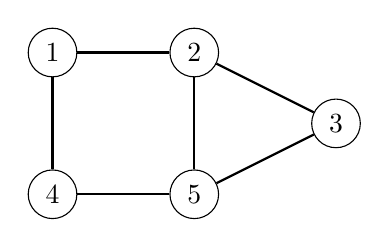
\begin{tikzpicture}[scale=0.9]
\node[draw, circle] (1) at (1,5) {$1$};
\node[draw, circle] (2) at (3,5) {$2$};
\node[draw, circle] (3) at (5,4) {$3$};
\node[draw, circle] (4) at (1,3) {$4$};
\node[draw, circle] (5) at (3,3) {$5$};

\path[draw,thick,-] (1) -- (2);
\path[draw,thick,-] (2) -- (3);
\path[draw,thick,-] (1) -- (4);
\path[draw,thick,-] (3) -- (5);
\path[draw,thick,-] (2) -- (5);
\path[draw,thick,-] (4) -- (5);
\end{tikzpicture}
\end{center}
包含一条从结点 1 到结点 3 的哈密顿路径：
\begin{center}
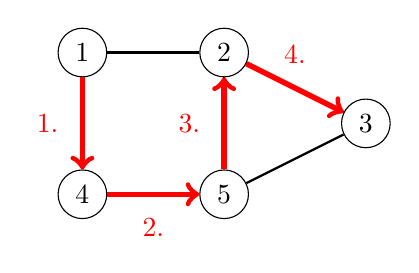
\begin{tikzpicture}[scale=0.9]
\node[draw, circle] (1) at (1,5) {$1$};
\node[draw, circle] (2) at (3,5) {$2$};
\node[draw, circle] (3) at (5,4) {$3$};
\node[draw, circle] (4) at (1,3) {$4$};
\node[draw, circle] (5) at (3,3) {$5$};

\path[draw,thick,-] (1) -- (2);
\path[draw,thick,-] (2) -- (3);
\path[draw,thick,-] (1) -- (4);
\path[draw,thick,-] (3) -- (5);
\path[draw,thick,-] (2) -- (5);
\path[draw,thick,-] (4) -- (5);

\path[draw=red,thick,->,line width=2pt] (1) -- node[font=\small,label={[red]left:1.}] {} (4);
\path[draw=red,thick,->,line width=2pt] (4) -- node[font=\small,label={[red]south:2.}] {} (5);
\path[draw=red,thick,->,line width=2pt] (5) -- node[font=\small,label={[red]left:3.}] {} (2);
\path[draw=red,thick,->,line width=2pt] (2) -- node[font=\small,label={[red]north:4.}] {} (3);
\end{tikzpicture}
\end{center}

\index{Hamiltonian circuit}

如果一条哈密顿路径的起点和终点是同一结点，就称它为\key{哈密顿回路}。上图还包含一条以结点 1 为起点和终点的哈密顿回路：
\begin{center}
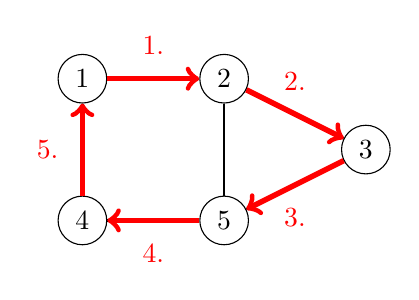
\begin{tikzpicture}[scale=0.9]
\node[draw, circle] (1) at (1,5) {$1$};
\node[draw, circle] (2) at (3,5) {$2$};
\node[draw, circle] (3) at (5,4) {$3$};
\node[draw, circle] (4) at (1,3) {$4$};
\node[draw, circle] (5) at (3,3) {$5$};

\path[draw,thick,-] (1) -- (2);
\path[draw,thick,-] (2) -- (3);
\path[draw,thick,-] (1) -- (4);
\path[draw,thick,-] (3) -- (5);
\path[draw,thick,-] (2) -- (5);
\path[draw,thick,-] (4) -- (5);

\path[draw=red,thick,->,line width=2pt] (1) -- node[font=\small,label={[red]north:1.}] {} (2);
\path[draw=red,thick,->,line width=2pt] (2) -- node[font=\small,label={[red]north:2.}] {} (3);
\path[draw=red,thick,->,line width=2pt] (3) -- node[font=\small,label={[red]south:3.}] {} (5);
\path[draw=red,thick,->,line width=2pt] (5) -- node[font=\small,label={[red]south:4.}] {} (4);
\path[draw=red,thick,->,line width=2pt] (4) -- node[font=\small,label={[red]left:5.}] {} (1);
\end{tikzpicture}
\end{center}

\subsubsection{存在条件}

目前没有已知的高效方法能够判断一个图是否包含哈密顿路径，而且该问题是 NP 困难的。不过在某些特殊情况下，我们可以确定图中一定存在哈密顿路径。

一个简单的观察是：如果图是完全图，即任意一对结点之间都有边，那么它一定包含哈密顿路径。此外，还有如下更强的结论：

\begin{itemize}
\item
\index{Dirac's theorem}
\key{Dirac 定理}：%\cite{dir52}
如果每个结点的度都至少为 $n/2$，则图中存在哈密顿路径。
\item
\index{Ore's theorem}
\key{Ore 定理}：%\cite{ore60}
如果每一对不相邻结点的度数之和都至少为 $n$，则图中存在哈密顿路径。
\end{itemize}

这些定理及其他相关结论有一个共同特征：当图中边的数量\emph{足够多}时，它们便能保证哈密顿路径存在。这很自然，因为图中的边越多，构造哈密顿路径的可能方式也就越多。

\subsubsection{构造}

既然没有高效方法能够判断哈密顿路径是否存在，那么显然也不存在高效构造该路径的方法；否则，只要尝试构造路径，就能判断它是否存在。

搜索哈密顿路径的一种简单方法是使用回溯算法，枚举构造路径的所有可能方式。此类算法的时间复杂度至少为 $O(n!)$，因为 $n$ 个结点共有 $n!$ 种不同的排列顺序。

一种更高效的解法基于动态规划（参见第 10.5 节）。其思想是计算函数 $\texttt{possible}(S,x)$ 的值，其中 $S$ 是结点集合的一个子集，$x$ 是其中一个结点。该函数表示是否存在一条访问 $S$ 中所有结点、并在结点 $x$ 结束的哈密顿路径。这一解法可以在 $O(2^n n^2)$ 时间内实现。

\section{De Bruijn 序列}

\index{De Bruijn sequence}

对于一个固定的、含 $k$ 个字符的字母表，\key{De Bruijn 序列}是这样一个字符串：每个长度为 $n$ 的字符串都恰好作为它的子串出现一次。这样的字符串长度为 $k^n+n-1$。例如，当 $n=3$、$k=2$ 时，一个 De Bruijn 序列为
\[0001011100.\]
该字符串的子串包含三位二进制串的所有组合：
000、001、010、011、100、101、110 和 111。

每个 De Bruijn 序列都对应某个图中的一条欧拉路径。构图方法是：每个结点表示一个长度为 $n-1$ 的字符串，每条边则向字符串添加一个字符。与上述情形对应的图如下：

\begin{center}
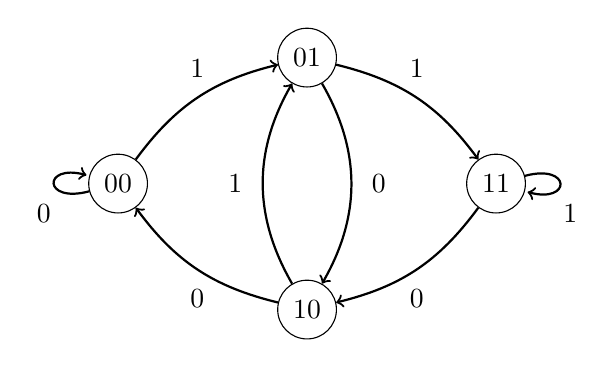
\begin{tikzpicture}[scale=0.8]
\node[draw, circle] (00) at (-3,0) {00};
\node[draw, circle] (11) at (3,0) {11};
\node[draw, circle] (01) at (0,2) {01};
\node[draw, circle] (10) at (0,-2) {10};

\path[draw,thick,->] (00) edge [bend left=20] node[font=\small,label=1] {} (01);
\path[draw,thick,->] (01) edge [bend left=20] node[font=\small,label=1] {} (11);
\path[draw,thick,->] (11) edge [bend left=20] node[font=\small,label=below:0] {} (10);
\path[draw,thick,->] (10) edge [bend left=20] node[font=\small,label=below:0] {} (00);

\path[draw,thick,->] (01) edge [bend left=30] node[font=\small,label=right:0] {} (10);
\path[draw,thick,->] (10) edge [bend left=30] node[font=\small,label=left:1] {} (01);

\path[draw,thick,-] (00) edge [loop left] node[font=\small,label=below:0] {} (00);
\path[draw,thick,-] (11) edge [loop right] node[font=\small,label=below:1] {} (11);
\end{tikzpicture}
\end{center}

该图中的一条欧拉路径对应一个包含所有长度为 $n$ 的字符串的字符串。这个字符串由起始结点中的字符以及各条边上的字符组成。起始结点含有 $n-1$ 个字符，边上共有 $k^n$ 个字符，因此字符串总长度为 $k^n+n-1$。

\section{骑士巡游}

\index{knight's tour}

\key{骑士巡游}是国际象棋中的骑士按照行棋规则，在 $n \times n$ 棋盘上移动并恰好访问每个方格一次的移动序列。如果骑士最终返回起始方格，就称为\emph{闭巡游}；否则称为\emph{开巡游}。

例如，下面是 $5 \times 5$ 棋盘上的一次开巡游：

\begin{center}
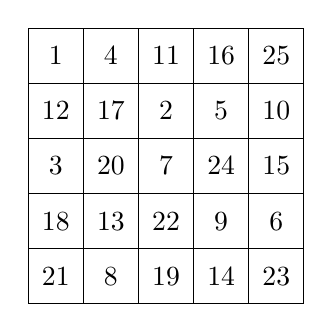
\begin{tikzpicture}[scale=0.7]
\draw (0,0) grid (5,5);
\node at (0.5,4.5) {$1$};
\node at (1.5,4.5) {$4$};
\node at (2.5,4.5) {$11$};
\node at (3.5,4.5) {$16$};
\node at (4.5,4.5) {$25$};
\node at (0.5,3.5) {$12$};
\node at (1.5,3.5) {$17$};
\node at (2.5,3.5) {$2$};
\node at (3.5,3.5) {$5$};
\node at (4.5,3.5) {$10$};
\node at (0.5,2.5) {$3$};
\node at (1.5,2.5) {$20$};
\node at (2.5,2.5) {$7$};
\node at (3.5,2.5) {$24$};
\node at (4.5,2.5) {$15$};
\node at (0.5,1.5) {$18$};
\node at (1.5,1.5) {$13$};
\node at (2.5,1.5) {$22$};
\node at (3.5,1.5) {$9$};
\node at (4.5,1.5) {$6$};
\node at (0.5,0.5) {$21$};
\node at (1.5,0.5) {$8$};
\node at (2.5,0.5) {$19$};
\node at (3.5,0.5) {$14$};
\node at (4.5,0.5) {$23$};
\end{tikzpicture}
\end{center}

骑士巡游对应于一个图中的哈密顿路径：图的结点表示棋盘方格，如果骑士能按照国际象棋规则在两个方格之间移动，就在对应的两个结点之间连边。

构造骑士巡游的一种自然方法是回溯。还可以使用\emph{启发式方法}引导骑士移动，使其尽快找到完整巡游，从而提高搜索效率。

\subsubsection{Warnsdorf 规则}

\index{heuristic}
\index{Warnsdorf's rule}

\key{Warnsdorf 规则}是一种寻找骑士巡游的简单而有效的启发式方法\footnote{这一启发式方法由 Warnsdorf 在 1823 年出版的著作 \cite{war23} 中提出。寻找骑士巡游也有多项式时间算法 \cite{par97}，但它们更为复杂。}。利用该规则，即使在很大的棋盘上也能高效构造巡游。其思想是：骑士每次都移动到后续可选步数\emph{尽可能少}的方格。

例如，在下图所示的局面中，骑士可以移动到五个方格（$a \ldots e$）：
\begin{center}
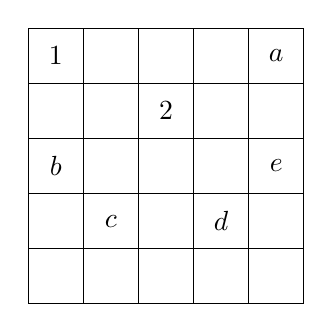
\begin{tikzpicture}[scale=0.7]
\draw (0,0) grid (5,5);
\node at (0.5,4.5) {$1$};
\node at (2.5,3.5) {$2$};
\node at (4.5,4.5) {$a$};
\node at (0.5,2.5) {$b$};
\node at (4.5,2.5) {$e$};
\node at (1.5,1.5) {$c$};
\node at (3.5,1.5) {$d$};
\end{tikzpicture}
\end{center}
在这种情况下，Warnsdorf 规则会把骑士移动到方格 $a$，因为作出该选择后，下一步只有一种可能。若选择其他方格，下一步都将有三种可能。
